\documentclass[11pt,compress,t,notes=noshow, aspectratio=169, xcolor=table]{beamer}

\usepackage{../../style/lmu-lecture}
% Defines macros and environments
% This file is included in slides and exercises

% Rarely used fontstyle for R packages, used only in 
% - forests/slides-forests-benchmark.tex
% - exercises/single-exercises/methods_l_1.Rnw
% - slides/cart/attic/slides_extra_trees.Rnw
\newcommand{\pkg}[1]{{\fontseries{b}\selectfont #1}}

% Spacing helpers, used often (mostly in exercises for \dlz)
\newcommand{\lz}{\vspace{0.5cm}} % vertical space (used often in slides)
\newcommand{\dlz}{\vspace{1cm}}  % double vertical space (used often in exercises, never in slides)
\newcommand{\oneliner}[1] % Oneliner for important statements, used e.g. in iml, algods
{\begin{block}{}\begin{center}\begin{Large}#1\end{Large}\end{center}\end{block}}

% Don't know if this is used or needed, remove?
% textcolor that works in mathmode
% https://tex.stackexchange.com/a/261480
% Used e.g. in forests/slides-forests-bagging.tex
% [...] \textcolor{blue}{\tfrac{1}{M}\sum^M_{m} [...]
% \makeatletter
% \renewcommand*{\@textcolor}[3]{%
%   \protect\leavevmode
%   \begingroup
%     \color#1{#2}#3%
%   \endgroup
% }
% \makeatother


\title{Interpretable Machine Learning}
% \author{LMU}
%\institute{\href{https://compstat-lmu.github.io/lecture_iml/}{compstat-lmu.github.io/lecture\_iml}}
\date{}

\bibliography{feature-importance}
%\usepackage{Sweave}
\begin{document}
	\newcommand{\titlefigure}{figure_man/feature-importance.png}
    \newcommand{\learninggoals}{
    	\item Underdstand how PFI is computed
    	\item Understanding strengths and weaknesses
    	\item Testing Importance}
	% Set style/preamble.Rnw as parent.
	
	% Load all R packages and set up knitr
	
	% This file loads R packages, configures knitr options and sets preamble.Rnw as 
	% parent file
	% IF YOU MODIFY THIS, PLZ ALSO MODIFY setup.Rmd ACCORDINGLY...
	
	% Defines macros and environments

	\lecturechapter{Permutation Feature Importance}
	\lecture{Interpretable Machine Learning}
	
	% ------------------------------------------------------------------------------

\begin{vbframe}{Permutation Feature Importance Idea}

In general, feature importance methods share two components
\lz
\begin{enumerate}
  \item \textbf{Perturbation/Removal:} Generate predictions for which the feature of interest has been perturbed/removed.
  \item \textbf{Performance Comparison:} Compare performance under perturbation/removal with the original model performance.
\end{enumerate}
\lz
\textbf{Permutation Feature Importance Idea:} "Remove" the feature of interest $x_j$ by perturbing it such that it is uninformative. Therefore, resample the variable from its marginal distribution $\P(x_j)$, e.g. by randomly permuting observations in $x_j$.

\footnote[frame]{\fullcite{Breiman2001rf}}

%\framebreak

%\begin{figure}
%  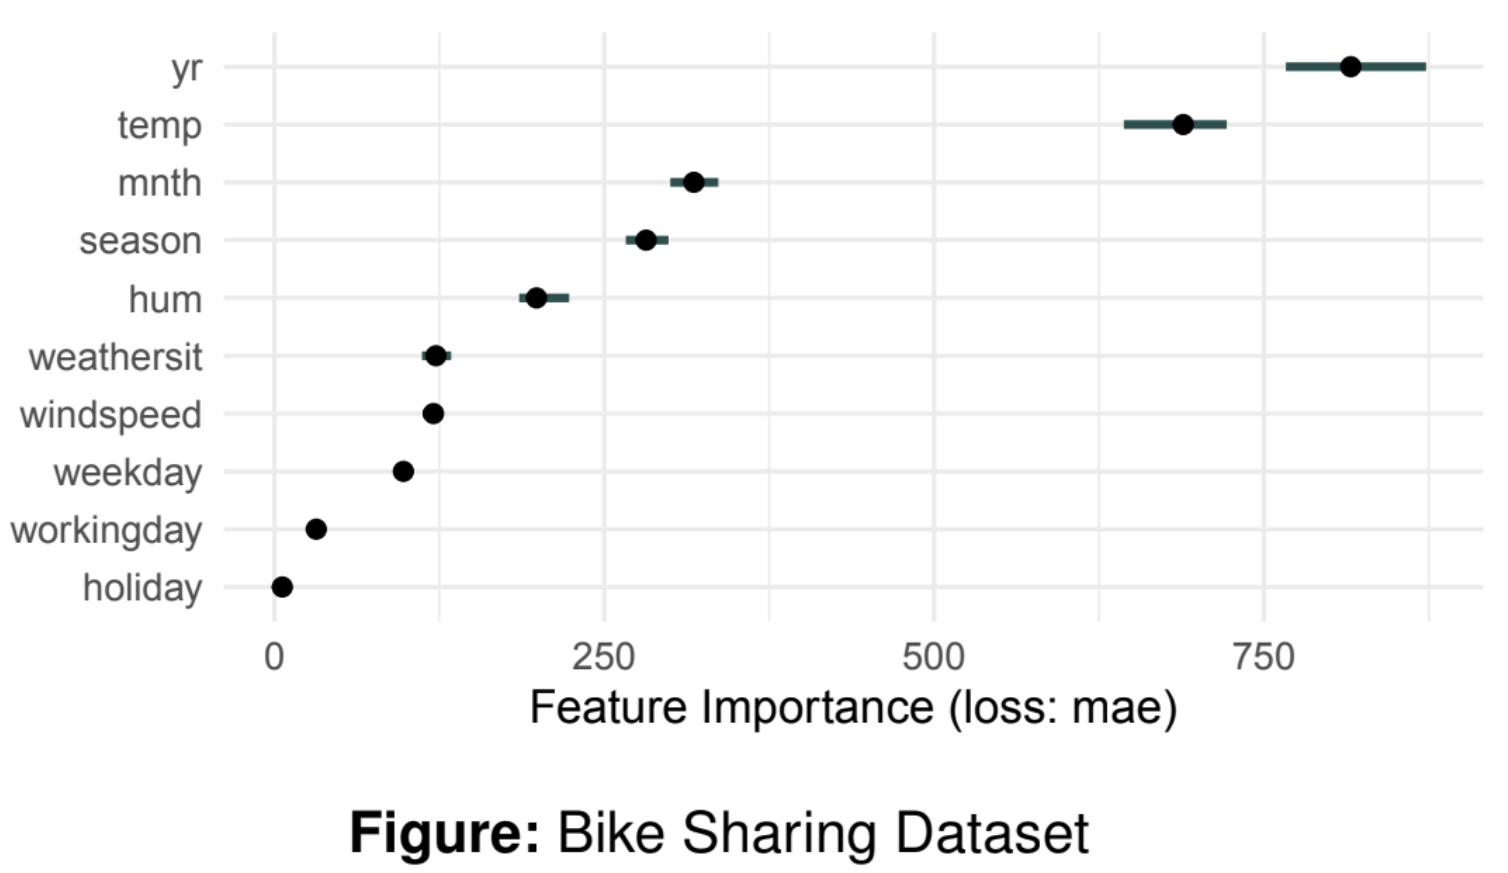
\includegraphics[width=0.75\textwidth]{figure_man/feature-importance.png}
%\end{figure}

%\vspace{-0.2cm}
%\tiny{Fisher et al. (2018). All models are wrong but many are useful: Variable importance for black-box, proprietary, or misspecified prediction models, using model class reliance. arXiv preprint arXiv:1801.01489 (2018).}

\end{vbframe}

\begin{vbframe}{Permutation Feature Importance}
\normalsize

Performance-based permutation feature importance (PFI) for features $x_S$ using test data $\D$:
\begin{itemize}
  \item Measure the error \color{red}\textbf{with permuted feature values} \color{black} $\pert{x}{}{}_S$
  \item Measure the error \color{blue}\textbf{without permuting features}\color{black}.
  \item Repeat permuting the feature (e.g., $m$ times) and average the difference of both errors: 
$$\widehat{PFI}_S = \tfrac{1}{m} \textstyle\sum\nolimits_{k = 1}^{m} \riske (\fh, {\color{red}\pert{\D}{S}{}_{(k)}}) - \riske (\fh, {\color{blue}\D})$$
\end{itemize}

The data $\D$ where $x_S$ is replace with $\pert{x}{S}{}$ is denoted as $\pert{\D}{S}{}$.\\
Example of permuting feature $x_S$ with $S = \{1\}$:

% TODO: update to new notation
\begin{center}
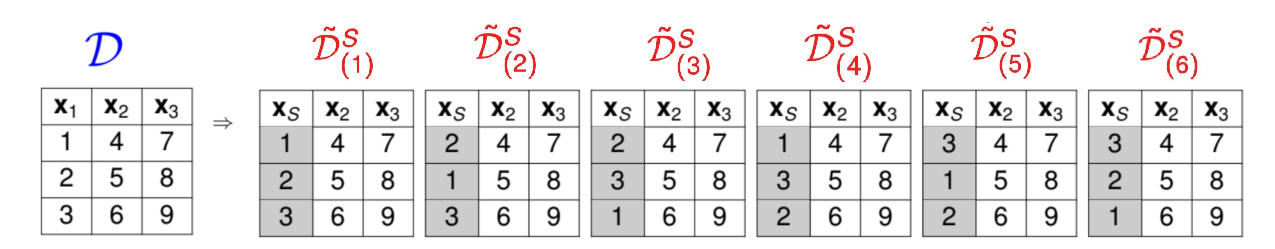
\includegraphics[width=0.75\textwidth]{figure_man/permuted-fv.pdf}
\end{center}

\vspace*{0.2cm}
{\scriptsize{Note: 
The $S$ in $x_S$ refers to a \textbf{S}ubset of features for which we are interested in their effect on the prediction.
As we calculate the feature importance for one feature at a time $|S| = 1$.}\par}

\end{vbframe}


\frame{

\frametitle{Permutation Feature Importance}

  \only<1-3,5-7>{$\hspace{36pt}{\color{white}\riske(\fh, {\color{red}\pert{\D}{S}{}_{(k)}}) - \riske(\fh, {\color{blue}\D})}$}
  \only<4>{$\hspace{36pt}\riske(\fh, {\color{red}\pert{\D}{S}{}_{(k)}}) - \riske(\fh, {\color{blue}\D}),$ where 
$\scriptstyle\riske(\fh, \D) =$ \scalebox{0.7}{$\frac{1}{n} \sum\nolimits_{(x, y) \in \D}$} $\scriptstyle L(\fh(x), y)$}
% $\scriptstyle\riske(\fh, \D) =$ \scalebox{0.7}{$\frac{1}{n} \sum\nolimits_{(x, y) \in \D}$} $\scriptstyle L(\fh(x), y)$}
%   \only<5-6>{$\hspace{36pt}{\color{white}\riske(\fh, {\color{red}\pert{\D}{S}{}_{(k)}}) - \riske(\fh, {\color{blue}\D})}$}
  
  \begin{center}
  \only<1>{\includegraphics[page=2, trim=0pt 5pt 0 66pt, clip, width=0.77\textwidth]{figure_man/pfi_demo2}}%
  \only<2>{\includegraphics[page=3, trim=0pt 5pt 0 66pt, clip, width=0.77\textwidth]{figure_man/pfi_demo2}}%
  \only<3-4>{\includegraphics[page=4, trim=0pt 5pt 0 66pt, clip, width=0.88\textwidth]{figure_man/pfi_demo2}}%
  \only<5>{\includegraphics[page=5, trim=0pt 5pt 0 66pt, clip, width=0.77\textwidth]{figure_man/pfi_demo2}}%
  \only<6>{\includegraphics[page=6, trim=0pt 5pt 0 66pt, clip, width=0.77\textwidth]{figure_man/pfi_demo2}}%
  \only<7>{\includegraphics[page=7, trim=0pt 5pt 0 66pt, clip, width=0.77\textwidth]{figure_man/pfi_demo2}}%
  \end{center}
  
  \begin{itemize}
    \only<1-2>{\item[1.]\textbf{Perturbation:} Sample feature values from the distribution of $x_S$ ($P(X_S)$). \newline $\Rightarrow$ Randomly permute feature $x_S$. Replace the original feature with the permuted feature $\pert{x}{}{}_S$ and create data with permuted feature   $\pert{\D}{S}{}$.}
    \only<2>{\item[2.] \textbf{Prediction:} Make predictions for both data, i.e., $\D$ and $\pert{\D}{S}{}$.}
    \only<3-4>{\item[3.] \textbf{Aggregation:}
      \begin{itemize}
        \item Compute the loss for each observation in both data sets.
      \end{itemize}}
    \only<5>{\item[3.] \textbf{Aggregation:}
      \begin{itemize}
        \item Compute the loss for each observation in both data sets.
       \item Take the difference of both losses $\Delta L$ for each observation.
      \end{itemize}}
     \only<6>{\item[3.] \textbf{Aggregation:}
      \begin{itemize}
        \item Compute the loss for each observation in both data sets.
        \item Take the difference of both losses $\Delta L$ for each observation.
        \item Average this change in loss across all observations.
      \end{itemize}}
    \only<7>{\item[3.] \textbf{Aggregation:}
      \begin{itemize}
        \item Compute the loss for each observation in both data sets.
        \item Take the difference of both losses $\Delta L$ for each observation.
        \item Average this change in loss across all observations.
        \item Also, average over multiple repetitions, if available.
      \end{itemize}}
  \end{itemize}
}

\begin{vbframe}{Bike Sharing Dataset}

\begin{center}
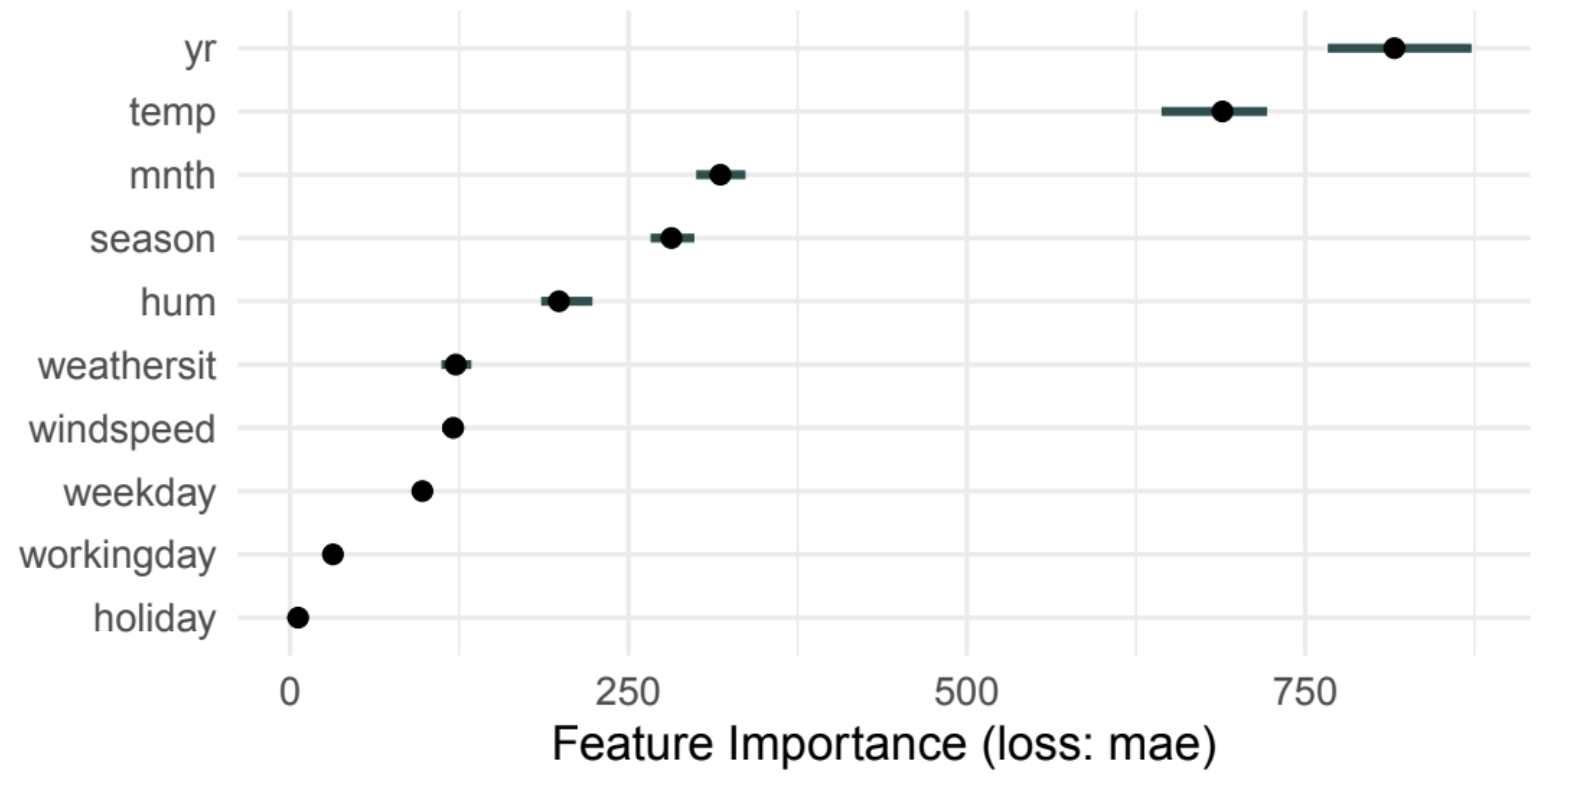
\includegraphics[width=0.66\textwidth]{figure_man/bike-sharing02.png}
\end{center}

\begin{itemize}
 \item The year is the most important feature. Features like weekday also contribute to the performance.
 \item Interpretation: Destroying the information about the year by shuffling this feature increases the mean absolute error of the model by an amount of 816.
 \item Additionally, the $5 \%$ and $95 \%$ quantile of the repetitions are shown as error bars.
\end{itemize}
\end{vbframe}

\begin{vbframe}{Permutation Feature Importance}
 \begin{itemize}
 \itemsep1em
  \item Interpretation: PFI displays the increase of the model error when the feature's information is destroyed.
  \item Results can be unreliable due to random permutations. \\
  $\Rightarrow$ Solution: Average results over multiple repetitions.
  \item Permuting features despite correlation with other features can lead to unrealistic combinations of feature values (since under dependence $\P(x_j,x_{-j}) \neq \P(x_j) \P(x_{-j})$).
  \item Feature importance automatically includes the importance of interaction effects with other features.
  \item The interpretation strongly depends on whether training or test data is used.\\
 \end{itemize}
\end{vbframe}

\begin{vbframe}{Permutation Feature Importance: Extrapolation}
 
 \textbf{Example:} Let $y = x_3 + \epsilon_y$ with $\epsilon_y \sim N(0, 0.1)$ where $x_1 :=  \epsilon_1$, $x_2 := x_1 + \epsilon_2$ are highly correlated ($\epsilon_1 \sim N(0,1), \epsilon_2 \sim N(0, 0.01)$) and $x_3 := \epsilon_3$, $x_4 := \epsilon_4$,  with $\epsilon_3, \epsilon_4 \sim N(0,1)$. All noise terms are independent.
A \texttt{lm} is fit, yielding $\fh(x) \approx 0.3 x_1 - 0.3 x_2 + x_3$.\\
 %
\begin{figure}
\hfill
  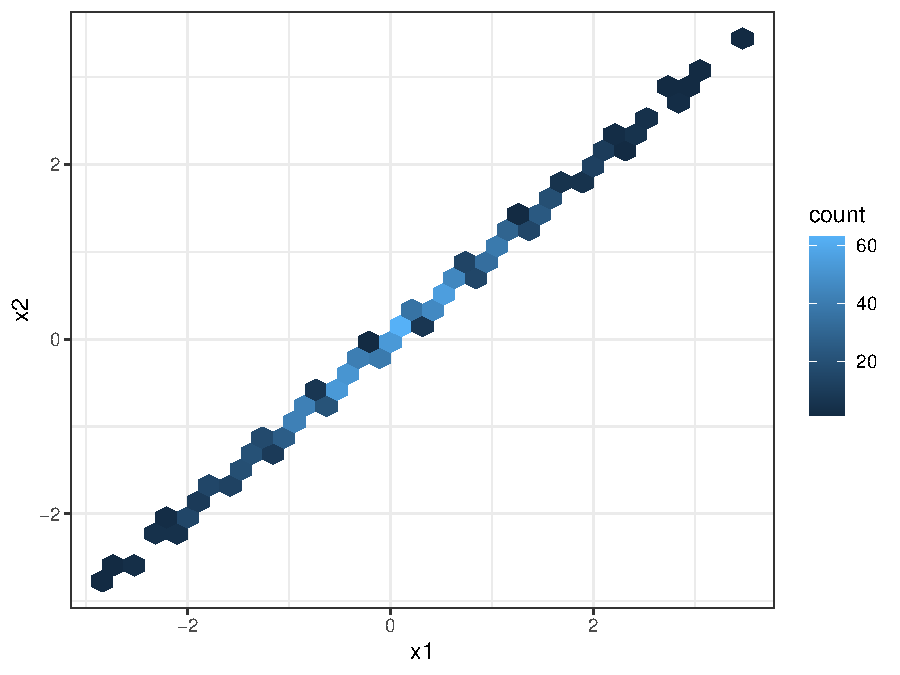
\includegraphics[width=0.25\linewidth]{figure_man/pfi_hexbin_pre.pdf}\hfill
  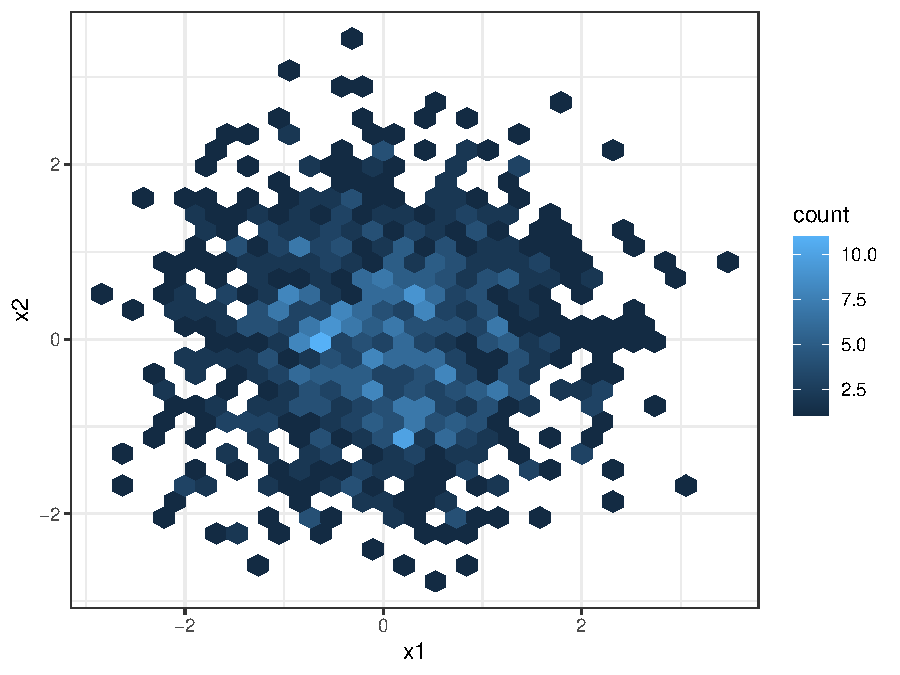
\includegraphics[width=0.25\linewidth]{figure_man/pfi_hexbin_post.pdf} \hfill
  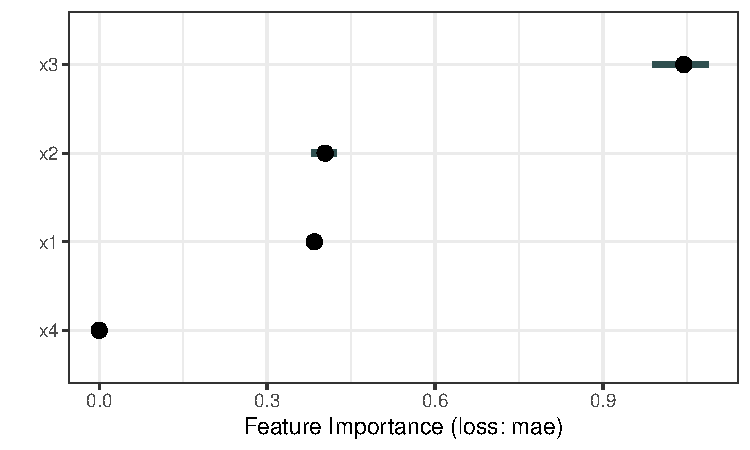
\includegraphics[width=0.4\linewidth]{figure_man/pfi_extrapolation.pdf} \hfill
  \caption{Density plot for $x_1, x_2$ before permuting $x_1$ (left) and after permuting $x_1$ (center). Right: PFI including $.05$ to $.95$ confidence band.}
\end{figure}
% 
$\Rightarrow$ $x_1$ and $x_2$ are irrelevant for the prediction for $\{x: \P(x) > 0\}$ \\
$\Rightarrow$ Since PFI evaluates the model on unrealistic observations, the features $x_1$ and $x_2$ are nevertheless considered relevant

 \end{vbframe}

\begin{vbframe}{Permutation Feature Importance: Interactions}

\textbf{Example:} Let $x_1, \dots, x_4$ be independently and uniformly sampled from $\{-1, 1\}$ and $y:= x_1 x_2 + x_3 + \epsilon_Y$ with $\epsilon_Y \sim N(0, 1)$.\\
A linear model is fit yielding $\fh(x) \approx x_1 x_2 + x_3$.\\

\begin{figure}
\centering
  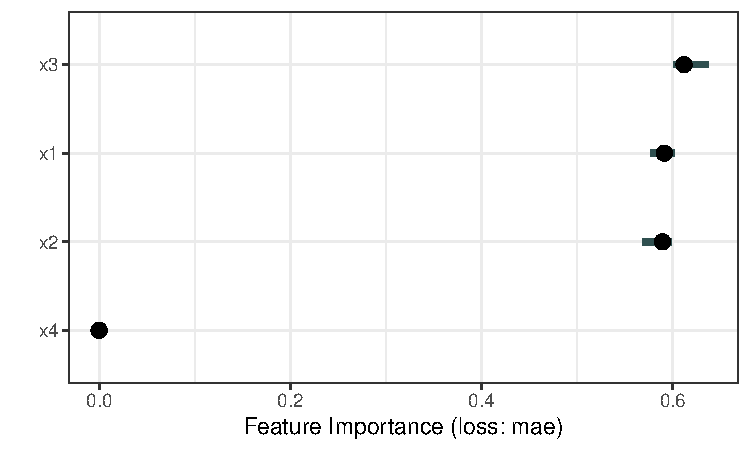
\includegraphics[width=0.5\linewidth]{figure_man/pfi_interactions.pdf}
\end{figure}

Although $x_3$ alone contributes as much to the performance as $x_1$ and $x_2$ jointly, all three are considered equally relevant.\\
\lz
$\Rightarrow$ PFI does not fairly attribute the performance to the individual features.
\end{vbframe}

\begin{vbframe}{Permutation Feature Importance: Test versus Training data}

\textbf{Example:} $x_1, \dots, x_{20}, y$ are independently sampled from $\mathcal{U} (-10, 10)$. A \texttt{xgboost} model with default hyperparameters if fit on a small training set of $50$ observations. The model overfits heavily.\\

\begin{figure}
  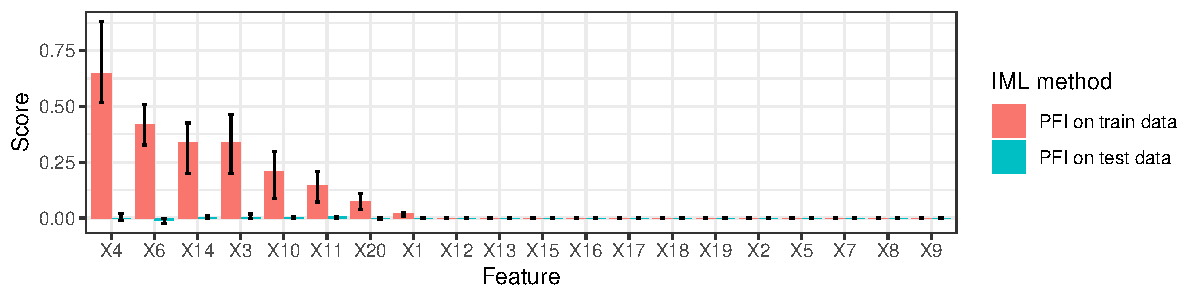
\includegraphics[width=0.6\linewidth]{figure_man/pfi_test_vs_train.pdf}
  \caption{While PFI on test data considers all features to be irrelevant, PFI on train data exposes the features on which the model overfit.}
\end{figure}

Why? PFI can only be nonzero if the permutation breaks a dependence in the data. Spurious correlations help the model perform on train data, but are not present in the test data.\\
$\Rightarrow$ If you are interested in which features help the model to generalize, apply PFI on test data.
  
\end{vbframe}

\begin{vbframe}{Implications of PFI}

Can we get insight into whether ...

\begin{enumerate}
    \item the feature $x_j$ is causal for the prediction?
    \begin{itemize}
      \item Nonzero PFI implies that the model relies on $x_j$.
      \item As the training vs test data example demonstrates, the contraposition does not hold.
    \end{itemize}
    \item the variable $x_j$ contains prediction-relevant information?
    \begin{itemize}
      \item Nonzero PFI implies that the feature is dependent with $y$ or it's covariates $x_{-j}$ or both (due to extrapolation).
      \item If a feature is not exploited by the model, PFI is zero, irrespective of whether the feature is useful or not.
    \end{itemize}
    \item the model requires access to $x_j$ to achieve it's prediction performance?    
    \begin{itemize}
      \item As the extrapolation example demonstrates, such insight is not possible.
\end{itemize}
\end{enumerate}
\end{vbframe}


\begin{vbframe}{Testing Importance (PIMP)}

\begin{itemize}
  \item PIMP was originally introduced for random forest feature importance.
  %\item It fixes the problem that the importance measure prefers features with many categories.
  \item PIMP investigates whether the PFI significantly differs from 0. 
  \item It computes the distribution of importances under the $H_0$-hypothesis that the feature is independent of the target $y$.
  \item Sampling under $H_0$ is achieved by permuting the $y$-vector and retraining the model.
  \item We now rescale the importance to a p-value - the tail probability under $H_0$ - as a new importance score.
\end{itemize}

\footnote[frame]{\fullcite{altmann2010permutation}}
%{\tiny{Altmann, André, et al. "Permutation importance: a corrected feature importance measure." 
%Bioinformatics 26.10 (2010): 1340-134.}}

\end{vbframe}

\begin{vbframe}{Testing Importance (PIMP)}

PIMP algorithm:
\begin{enumerate}
	\item For $m \in \{1, \ldots, n_{repetitions}\}$:
		\begin{itemize}
			\item Permute response vector $y$.
			\item Retrain model with data $\Xmat$ and permuted $y$.
			\item Compute feature importance $PFI_j^m$ for each feature $j$.
		\end{itemize}
	\item Train model with $\Xmat$ and unpermuted $y$.
	\item For each feature $j \in \{1,\ldots,p\}$:
		\begin{itemize}
			\item Fit probability distribution of the feature importance values $PFI_j^m$, $m \in \{1, \ldots, n_{repetitions}\}$ (choice between Gaussian, lognormal, gamma or non-parametric).
			\item Compute permutation feature importance $PFI_j$ for the model without permutation.
			\item Retrieve the p-value of $PFI_j$ based on the fitted distribution.
		\end{itemize}
\end{enumerate}
\end{vbframe}

\begin{vbframe}{Excurs: Multiple testing problem}
\begin{itemize}
  \item When should we reject the $H_0$-hypothesis for a feature? 
  \item The larger $p$, the more tests need to performed by PIMP. 
  \item This can lead to the \textbf{multiple testing problem}: If one does not take the multiplicity of tests into account, then the probability that some of the true null hypotheses are rejected (type-I error) by chance alone may be unduly large.
  \item Accounting for multiplicity of individual tests can be achieved by controlling
  an appropriate error rate like the \textbf{familywise error rate} (FWE, the probability of at least one type-I error). 
  \item One classical method to control the FWE is the \textbf{Bonferroni correction} which rejects a null hypothesis if its p-value is smaller than $\alpha/p$ with $p$ as the number of tests. 
  \item We refer to other lectures like \textit{Schätzen \& Testen I} for more details.
  \end{itemize} 

  \footnote[frame]{\fullcite{romano2010multiple}}
  %{\tiny{Romano, J. P., Shaikh, A. M., and Wolf, M. (2010). Multiple Testing. The New Palgrave Dictionary of Economys. \url{https://home.uchicago.edu/~amshaikh/webfiles/palgrave.pdf}}\par}
\end{vbframe}

\begin{vbframe}{PIMP for extrapolation example}
\textbf{Recap:} $x_1$ and $x_2$ are highly correlated by independent of $y$. $x_4$ is independent of all other variables, $x_3$ is only correlated with $y$.\\
A \texttt{lm} is fit, yielding $\fh(x) \approx 0.3 x_1 - 0.3 x_2 + x_3$.\\
 %
\begin{figure}
  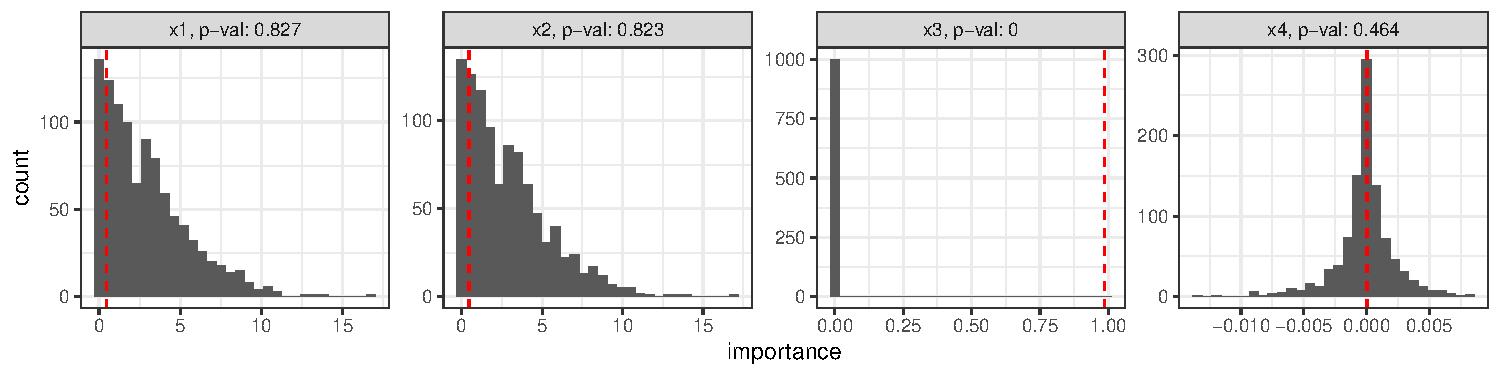
\includegraphics[width=0.45\linewidth]{figure_man/pimp.pdf}
  \caption{$H_0$ distribution (100 samples) for each feature as histograms, the true PFI indicated in red. PIMP only considers $x_3$ relevant. Although PFI for $x_1$ and $x_2$ is nonzero, PIMP considers them irrelevant since they are not predictive of $y$. Even after permuting $y$, the model relies on them.}
\end{figure}
\end{vbframe}

\begin{vbframe}
  \printbibliography
\end{vbframe}

\endlecture
\end{document}
